\scanpage{100}

Tangentes \inserted{aux composantes irréductibles} de $M'_3$ \uline{en $a$} sont \deleted{\unsure{distinctes}} égales. \deleted{$G'$ \unsure{opère sur}} \inserted{L'espace} tangent à $M_3$ en $a$ splitte canoniquement en $V_1\times V_2$, avec $V_1$ vertical (espace tangent à $(M_3)_b$) et $V_2$ horizontal, et $G'$ opère \unsure{trivialemt|trivialem} sur $V_2$, et laisse $V_1$ stable. donc $G'$ opère via $\mathbb F_4^*\inserted{\simeq\mathbb Z/3\mathbb Z}$ sur $V_1$. Or, \deleted{\unsure{la|les}} théorie de la ramification en car. 2 nous dit précisément [l'action de $G'$ sur $(M_3)_2$ étant \deleted{\unsure{fidèle, que}}\inserted{fidèle}) que le noyau de \deleted{la partie stable de} \unsure{ordres|est très} vraisemblablement précisément le 2-sous-groupe invariant \inserted{$P'$} de $G'$, qui est d'ordre 8, \deleted{\unsure{et dès}} que l'image \deleted{\unsure{étant}} \unsure{être|est} d'ordre \deleted{\unsure{card}} $[G':P']=3=\operatorname{card}\mathbb F_4^*\simeq\mathbb Z/3\mathbb Z$. Par suite, on trouve que $G'\to\mathbb F_4^*$ est surjectif, et déterminé à priori ``au signe près'' [i.e via autom. du \inserted{groupe} $\mathbb Z/3\mathbb Z$] Il faudrait encore déterminer lequel\deleted{\unsure{lement|que}} c'est.

\margin{\figure{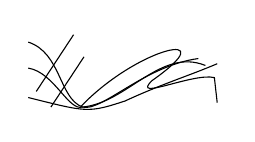
\begin{tikzpicture}[x=.6cm,y=.55cm]
\draw (0,1.5) .. controls (.7,1.25) and (.65,.2) .. (1.15,0) .. controls (1.55,-.12) and (2.45,.95) .. (3.6,1.12);
\draw (0,.9) .. controls (.55,.8) and (.85,-.1) .. (1.15,0) .. controls (2.1,.1) and (2.8,1.38) .. (3.75,.96);
\draw (0,.22) .. controls (1.25,-.12) and (1.26,-.14) .. (2.05,.14) .. controls (2.82,.53) and (3.42,.73) .. (4,1);
\draw (.17,.36)--(.96,1.67) (.48,0)--(1.18,1.16) (1.12,.02).. controls (2.36,1.42) and (4.2,1.82)..(2.62,.61).. controls (2.16,.12) and (3.5,.8)..(3.94,.68)--(4,.1);
\end{tikzpicture}}}

\uline{Attention}, $\mu_3$ \uuline{n'opère pas} sur la courbe modulaire $\mathbb E$ sur $M'_3$, \deleted{en s'y \unsure{opérant}} \inserted{en prolongeant son} action au dessus de $M'_3[\frac13]$. Car \deleted{\unsure{alors on}} son \deleted{\unsure{en remarquant que son action sur}} action commuterait à celle de $G$, \deleted{\unsure{donc} qui \unsure{serait} l'action résiduelle par $\mu_6$ \unsure{serait}, donc fidèle en tt point, \unsure{on en sait que|ce fait sait que} le gpe des autom. \deleted{\unsure{est}} à fibres étales, donc sa fibre chez le point 2 un point \unsure{contient} $\mu_6=\underset{\text{radical}}{\mu_2}\times\mu_3$. Par contre, \inserted{$=\mu_6$} $\mu_3$ opère sur la $\mathbb Z/6\mathbb Z=B$ opère sur \unsure{$E$} tte \unsure{courbe} elliptique en opérant sur \unsure{$E$} \unsure{au de façon} canoniquement pour la \unsure{raison}, $E$ sur une base de car. résiduelle $\ne3$,} donc on a on aurait action de $\mu_3$ et $G'$ sur $E_a$, et comme $G'=\mathrm{Aut}(E_a)$, il s'ensuivrait que $\mu_3\subset G'$ est $\mu_3$ dans le centre de $G'$. Or le 3-sous-groupe de Sylow \deleted{\unsure{du}} de $G'$ \uline{n'est pas central} ! // Ceci impose des restrictions \deleted{\unsure{sur les}}\inserted{aux} raccords des composantes de $M'_3$. \deleted{\unsure{La seule}} \inserted{groupe des} autom. \unsure{automorphismes} de $E$ sur $M'_3$ est donc $\mathbb Z/2\mathbb Z$, \unsure{par} \deleted{$\mathrm{Sl}(2,\unsure{\mathbb Z/3\mathbb Z})/\unsure{\mu_2|\mu_3}$ \unsure{opère fidèlement sur} $M'_3$} qui est aussi le grpe noyau de \deleted{\unsure{sur}} l'opération de $\mathrm{Sl}(2,\mathbb Z/3\mathbb Z)=G'$, sur $M'_3$.

\margin{\figure{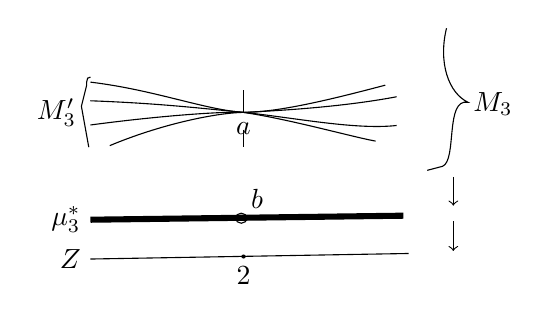
\begin{tikzpicture}[x=.72cm,y=.64cm]
\draw (0,2.82).. controls (1.12,2.67) and (2.02,2.27)..(2.7,2.22).. controls (3.36,2.22) and (4.42,2.53)..(5.2,2.76);
\draw (0,2.45).. controls (1.22,2.40) and (1.95,2.3)..(2.7,2.22).. controls (3.65,2.27) and (4.6,2.36)..(5.4,2.53);
\draw (0,1.97).. controls (1.2,2.15) and (2.3,2.24)..(2.7,2.22).. controls (3.62,2.11) and (4.68,1.87)..(5.4,1.96);
\draw (.34,1.56).. controls (1.23,1.98) and (2.2,2.21)..(2.7,2.22).. controls (3.53,2.08) and (4.63,1.73)..(5.03,1.65);
\draw (2.7,2.66)--(2.7,2.23) (2.7,1.88)--(2.7,1.54);
\node[below] at (2.7,2.22){$a$};
\draw (0,2.92).. controls (-.1,2.94) and (-.05,2.73)..(-.08,2.7)--(-.16,2.34)--(-.03,1.53);
\node[left] at (-.08,2.22){$M'_3$};
\draw (6.28,3.89).. controls (6.13,3.2) and (6.32,2.6)..(6.66,2.42).. controls (6.25,2.51) and (6.47,1.27)..(6.21,1.15)--(5.94,1.07);
\node[right] at (6.58,2.38){$M_3$};
\draw[line width=2.2pt] (0,.09)--(5.52,.17);
\draw (2.66,.12) circle (.1);
\node[above right] at (2.66,.12){$b$};
\node[left] at (0,.09){$\mu_3^*$};
\draw (0,-.69)--(5.61,-.58);
\fill (2.70,-.64) circle (.04);
\node[below] at (2.70,-.64){$2$};
\node[left] at (0,-.69){$\mathbb Z$};
\draw[->] (6.4,.94)--(6.4,.37);
\draw[->] (6.4,.06)--(6.4,-.53);
\end{tikzpicture}}}
% archive sheet number: 99
